Overview (0.5 page) (AJ, JP)
\begin{itemize}
  \item "Technical Part" (AJ)
  \item SES
  \item Cavity
  \item Ray-casting + parameters for vis
\end{itemize}

\subsection{Overview}

Overview of the algorithm: (JP)
\begin{itemize}
  \item Per frame we perform the following steps: ...
  \item The data comes in form of trajectories describing motion of individual atoms, we do not assume anything about the data.
  \item We split computations to two groups, which are performed on per frame basis.
	\begin{enumerate}
	  \item Data preprocessing (surface, cavity and attributes computations)
		\item Visualization  (ray-casting, opacity calculation, etc.)
	\end{enumerate}
\end{itemize}

\begin{figure}[htb]
  \centering
  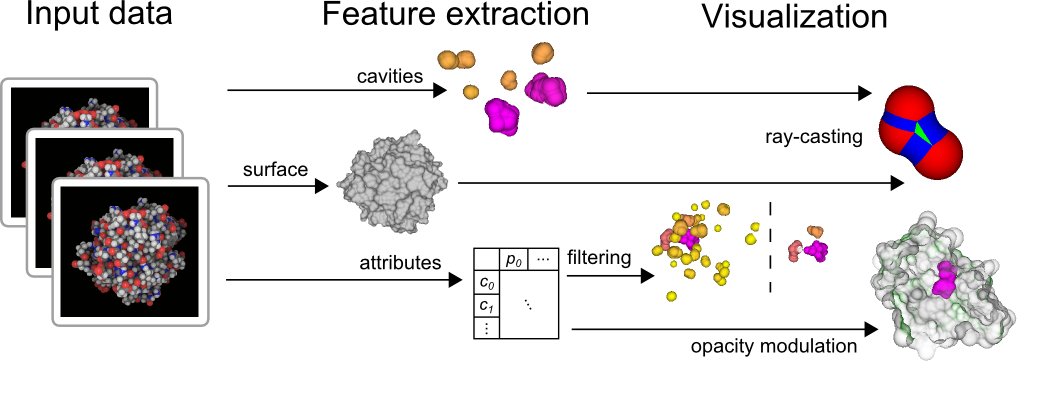
\includegraphics[width=3.3in]{image/overview.png}
  \caption{\textcolor{red}{TODO}.}
	\label{fig:overview}
\end{figure}

\begin{figure}[htb]
  \centering
  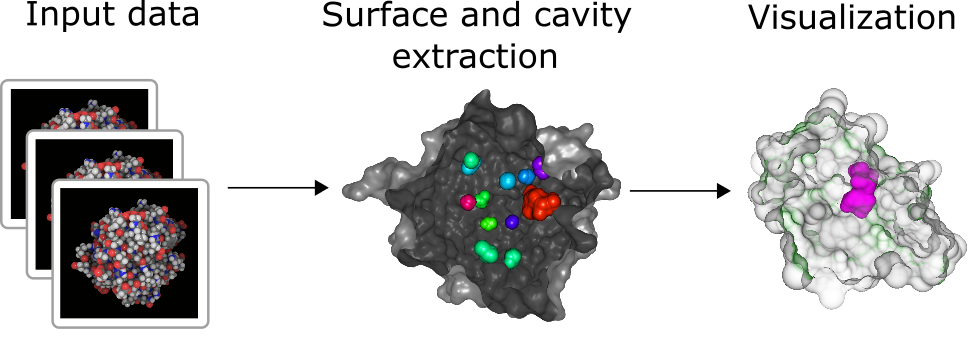
\includegraphics[width=3.3in]{image/overview2.png}
  \caption{\textcolor{red}{TODO}.}
	\label{fig:overview2}
\end{figure}

\subsection{Extended CB Algorithm}

We come out from the GPU parallel algorithm presented in \cite{krone2011parallel}.
In the algorithm, the SES is represented as three different sets of surface primitives --- spheres, tori\textcolor{red}{,} and spherical triangles, that are ray-casted to obtain opaque surface visualization.
While ray-casting spheres and tori, there are also produced parts that are in the final image occluded by triangles.
Therefore, to visualize contour surface representation using transparency, we extended the algorithm so that it computes a SES represented with:
\begin{itemize}
  \item Spherical patches --- a spherical patch is enclosed by edges of three or more toroidal patches.
	\item Toroidal patches --- a toroidal patch is delimited by two spherical triangles.
	\item Spherical triangles.
\end{itemize}

In \cite{kauker2013rendering}, the authors shown that a toroidal patch can be ray-casted using a torus and two clipping planes defined by its delimiting triangles.
We modified the data structure used to store spherical triangles in a way, such that we know all spherical triangles that delimit patches on a torus and hence later on we are able to ray-cast toroidal patches instead of tori.
In order to get all triangles incident to some torus, we hash the triangles by three keys --- one for each torus which is connected to a triangle.
We implemented a simple hash table which is based on linear addressing scheme with quadratic probing.
For more details regarding the hashing technique see \cite{alcantara2011efficient}.

Since a spherical patch is bounded by toroidal patches, we extended the original algorithm by adding three new GPU kernels that compute sets of toroidal patches forming spherical patches (see Section~\ref{sec:graph}). When visualizing the surface, each such set is used to ray-cast a spherical patch (see Section~\ref{sec:spherical-patches}).

\begin{figure}[htb]
  \centering
  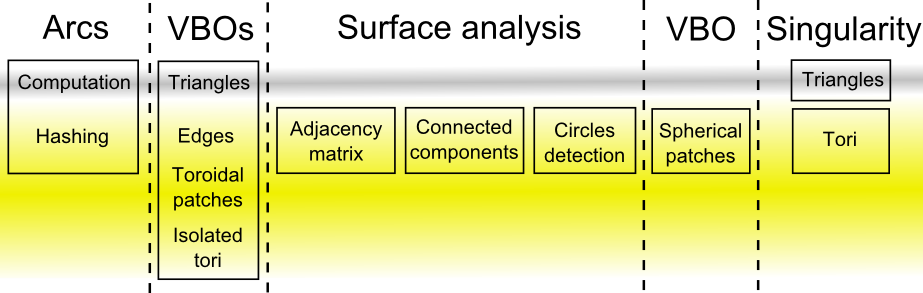
\includegraphics[width=3.3in]{image/kernels.png}
  \caption{Overview of our extended algorithm.
	The algorithm steps are ordered from the left to the right.
	GPU kernels are marked with squares containing both original (grey) and our novel parts (yellow).}
	\label{fig:kernels}
\end{figure}

\subsection{Surface graph}
\label{sec:graph}

\textbf{This should be written in more friendly fashion and with clear defined terms.
Terms to be explained: surface is continuitous (geometrical?, since $C^1$ continuous it is not), graphs (2D/3D, does it contain loops?), primitive, component }   
\begin{itemize}
  \item Idea: computed surfaces are continuous (closed) and graphs of their primitives form isolated components in the whole graph of all surface primitives
  \item Modification of parallel CB of Krone et. al --- aaaa
  \item Extension of parallel CB of Krone et. al --- 3 new kernels:
	\begin{enumerate}
	  \item Adjacency matrix is built (only 3 edges at each vertex)
    \item Labeling of connected components (parallel BFS --- suboptimal)
    \item Circles of edges for each spherical patch are computed
  \end{enumerate}
  \item Assign spheres with edges
  \item Detect circles in edges --- bubble sort $O(n^2)$
  \item Step 3 --- one sphere can form two or more surfaces
  \item Rendering of spherical patches --- spherical polygons
  \item Odd-even rule + point outside polygon
  \item Special case: isolated tori
\end{itemize}

Seeds --- The computed surface contains also surface of cavities that was inaccurately called by Kauker et. al. as inner remains \cite{kauker2013rendering}.
For SES, the user might want to visualize cavities within the molecular surface.
Contrary, for SAS, the inner surface forms only \textcolor{red}{seeds} of the cavities, and the seeds are not useful for assessing the real shape of a cavity, so that clipping these seeds enhances the visualization.
The user might also want to hide cavities inside a SES to lower possible occlusion of other structures such as tunnels or cartoons.
The clipping of cavities is enabled by observing that both SAS and SES are continuous and therefore there has to be more than one continuous surface component when the molecule contains a cavity \cite{borland2011ambient}.
\textcolor{red}{Too many ideas in one sentence. Split into two or more.}

\textcolor{red}{Introduce here "terminus techniques"; i.e., SES is composed of three types of patches etc.}
More precisely, there is one component for the outer surface of the molecule and one component for each cavity, and the components can be easily detected by applying connected component (CC) analysis to the graph formed by surface primitives (spherical patches --- polygons?, toroidal patches and triangles).
The spherical patches \textcolor{red}{can not be used because they are not known for now}.
We do not know whether a sphere forms one or more patches and who are their neighboring tori, i.e., edges.
Therefore the surface graph is built by triangles (vertices) and toroidal patches (edges).
The surface contains also tori that are not cut by any triangle, i.e., they do not have any neighboring triangle.
Such toroidal patches are excluded from the surface graph and has to be handled differently (see Section ?).

We do the CC analysis on the GPU to avoid synchronization and data transfer costs.
First, we modified the output of the original GPU parallel CB to obtain the input which is needed for the analysis and rendering of transparent toroidal patches.
In the original algorithm \cite{krone2011parallel}, an arc intersection was stored only for atoms whose indices fulfilled $i < j < k$.
This is insufficient for rendering the toroidal patches transparent as they can't be rendered as a one whole patch because the parts that would be hidden by the opaque surface would be visible.
Instead, we split each torus into its visible patches based on their neighboring triangles that delimit them.
Since each torus is defined by a small circle between atoms $i$ and $j$, we are interested in all triangles that were produced by atoms $i$, $j$ and some other atom $k$.
For this purpose, we store the computed arc intersections in a linear buffer (employing atomics) and together produce a hash structure which enables us to find the triangles by their two of the three atom indices.
As a benefit to this hash structure, we save GPU memory because the original arcs structure was very sparse.
Now, we store n arcs together with $3 n$ keys in a hash table which data/free ratio is 2. \textcolor{red}{TODO: More precision.}

The analysis part is split into three steps and for each we implemented one GLSL compute shader.
First, the adjacency matrix of the surface graph is computed.
The matrix will have one row for each vertex and three columns, because each triangle has exactly (at most?) three neighbouring toroidal patches in the surface. In the next step, all connected components are detected and labeled using BFS.
Our implementation of the BFS algorithm is suboptimal, because its time complexity is $O(d \cdot n)$ where d is the length of the longest shortest path among all vertices in a component.
In the worst case, d can be n.
The reason we choose such ineffecient implementation was the ability of BFS implementation in one compute shader \cite{merrill2012scalable}.
Our decision is also supported by performance measures (see Section \textcolor{red}{?}) where the computation of labels takes only ~5 ms for a molecule with ~10000 atoms while the computation of SES takes 5x more.
Finally, we sort all edges neighboring with a sphere to get one or more circles where each circle delimits a spherical path.
The lables for the spherical pathes are obtained from the labels of some of their delimiting edges.

\subsection{Special case --- isolated tori}

These tori must be handled in two way.
First, the label of the surface that an isolated tori forms must be found --- recall, the tori is not part of the surface graph.
Second, each isolated tori should clip overlaid fragments of its spherical patch (see Figure \textcolor{red}{?}).

%\begin{equation}
% \sum_{j=1}^{z} j = \frac{z(z+1)}{2}
%\end{equation}

%\paragraph{Rejected Ejector Seat Reservation}